%!TEX root = article.tex

\section{Appendix}
\label{s:Appendix}

Additional material such as extra figures.
\subsection{DuMuX Results Visualized with ParaView}
%Put all the extra images from ParaView here.
\begin{figure}[h]
\centering
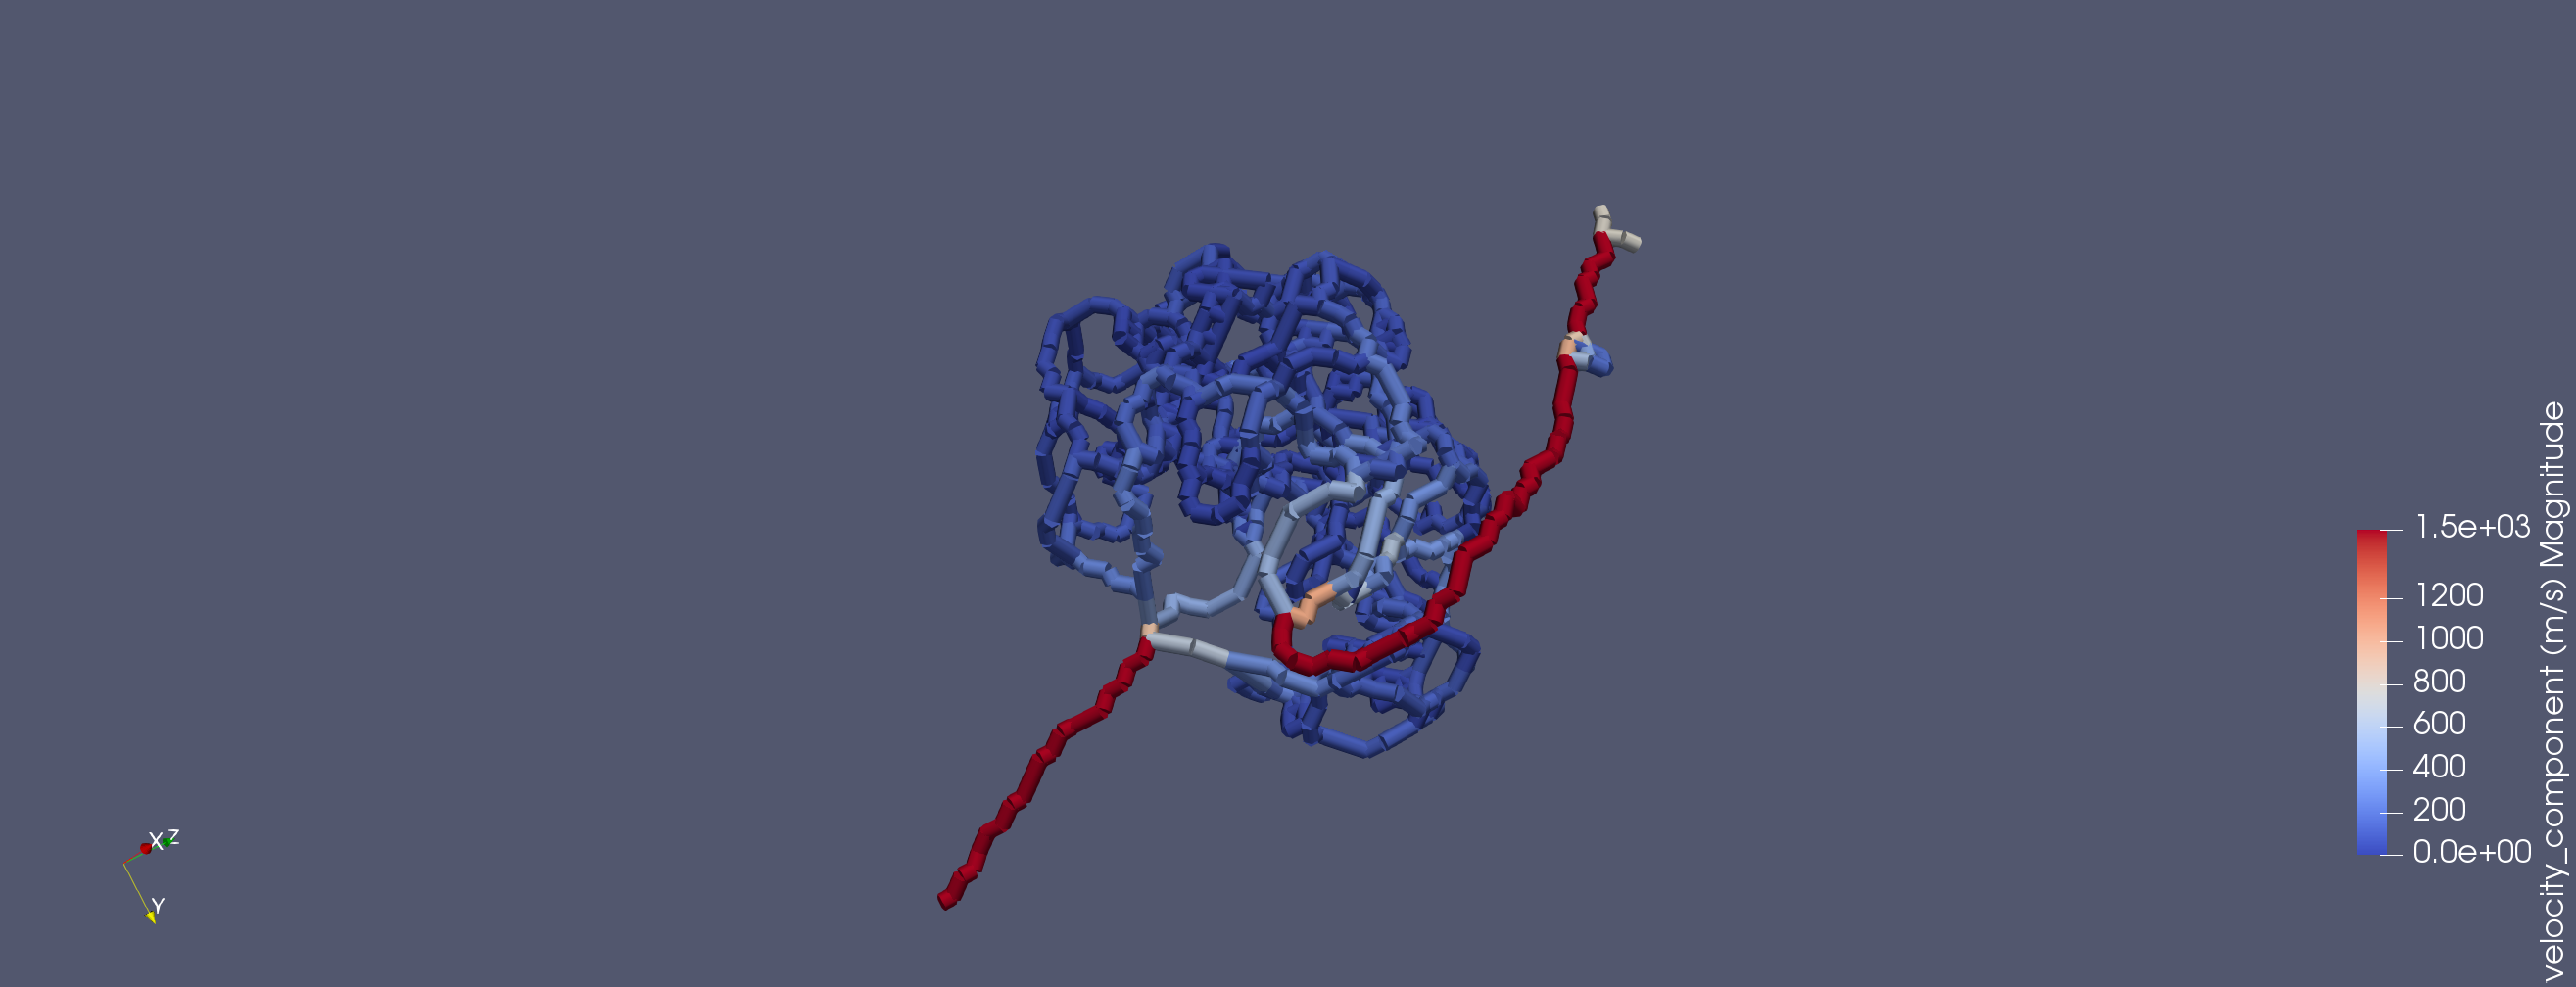
\includegraphics[width=162mm]{nephron_velocity}
\caption{Velocity Field in a Nephron}
\label{fig:nephron_velocity}
\end{figure}
The figure \ref{fig:nephron_velocity} is the result of a DuMuX 1p-1p blood flow simulation computed on a nephron network. The velocity field of the flow is visualized.\\

\begin{figure}[h]
\centering
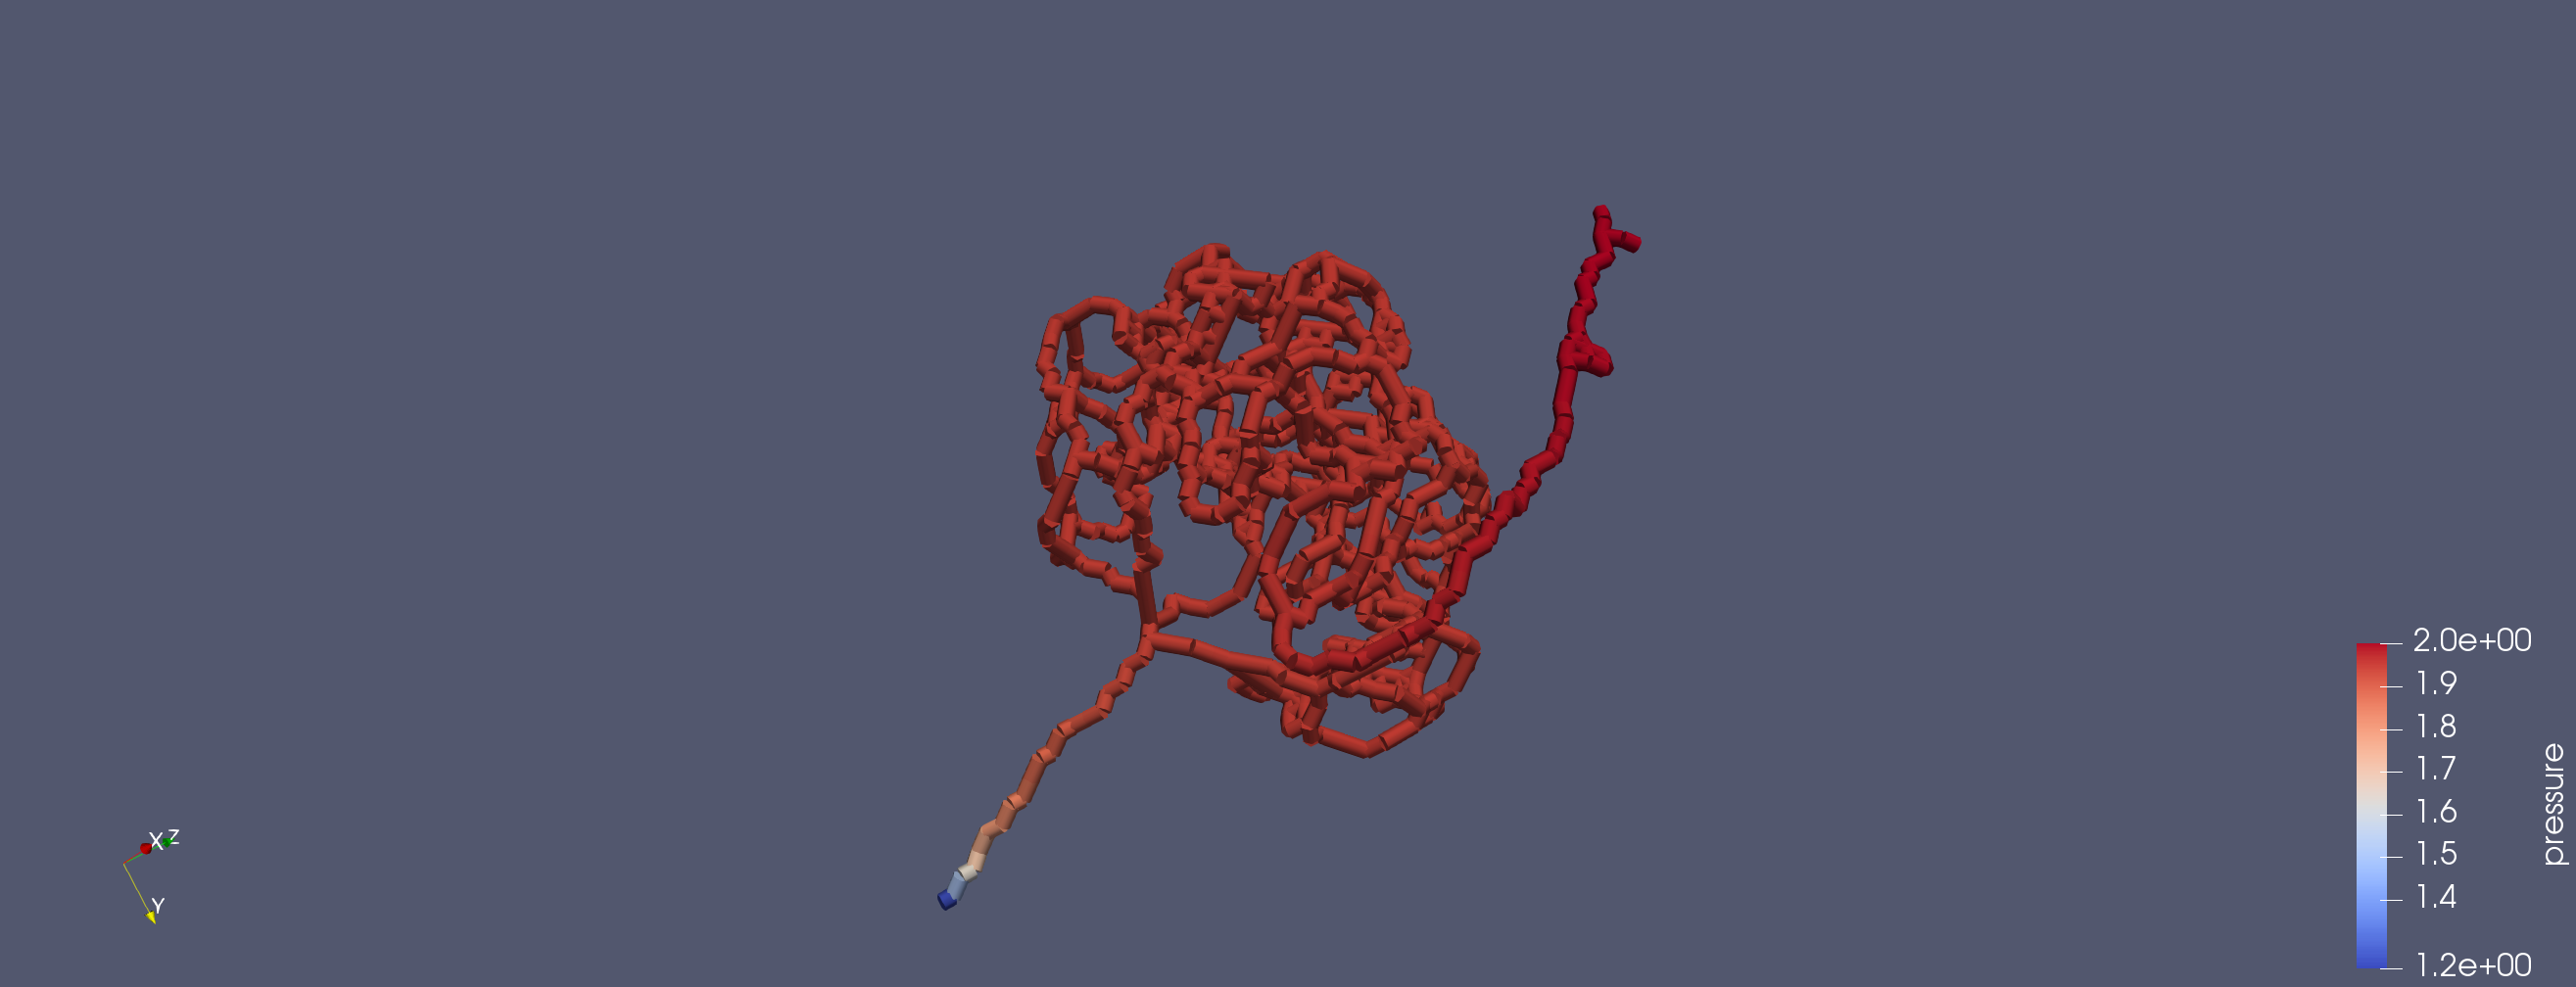
\includegraphics[width=162mm]{nephron_pressure}
\caption{Pressure Field in a Nephron}
\label{fig:nephron_pressure}
\end{figure}
The figure \ref{fig:nephron_pressure} is the result of a DuMuX 1p-1p blood flow simulation computed on a nephron network. The pressure field of the flow is visualized.\\

\subsection{Green's Function Code Results}
%Put all the extra plots etc. from Green's Function Code here.

Figure \ref{fig:Contour_Cardiac}  is the result of a Green's Method blood flow simulation computed on a Cardiac network. The Solute Concentration in the network is visualized.\\
\begin{figure}[h]
\centering
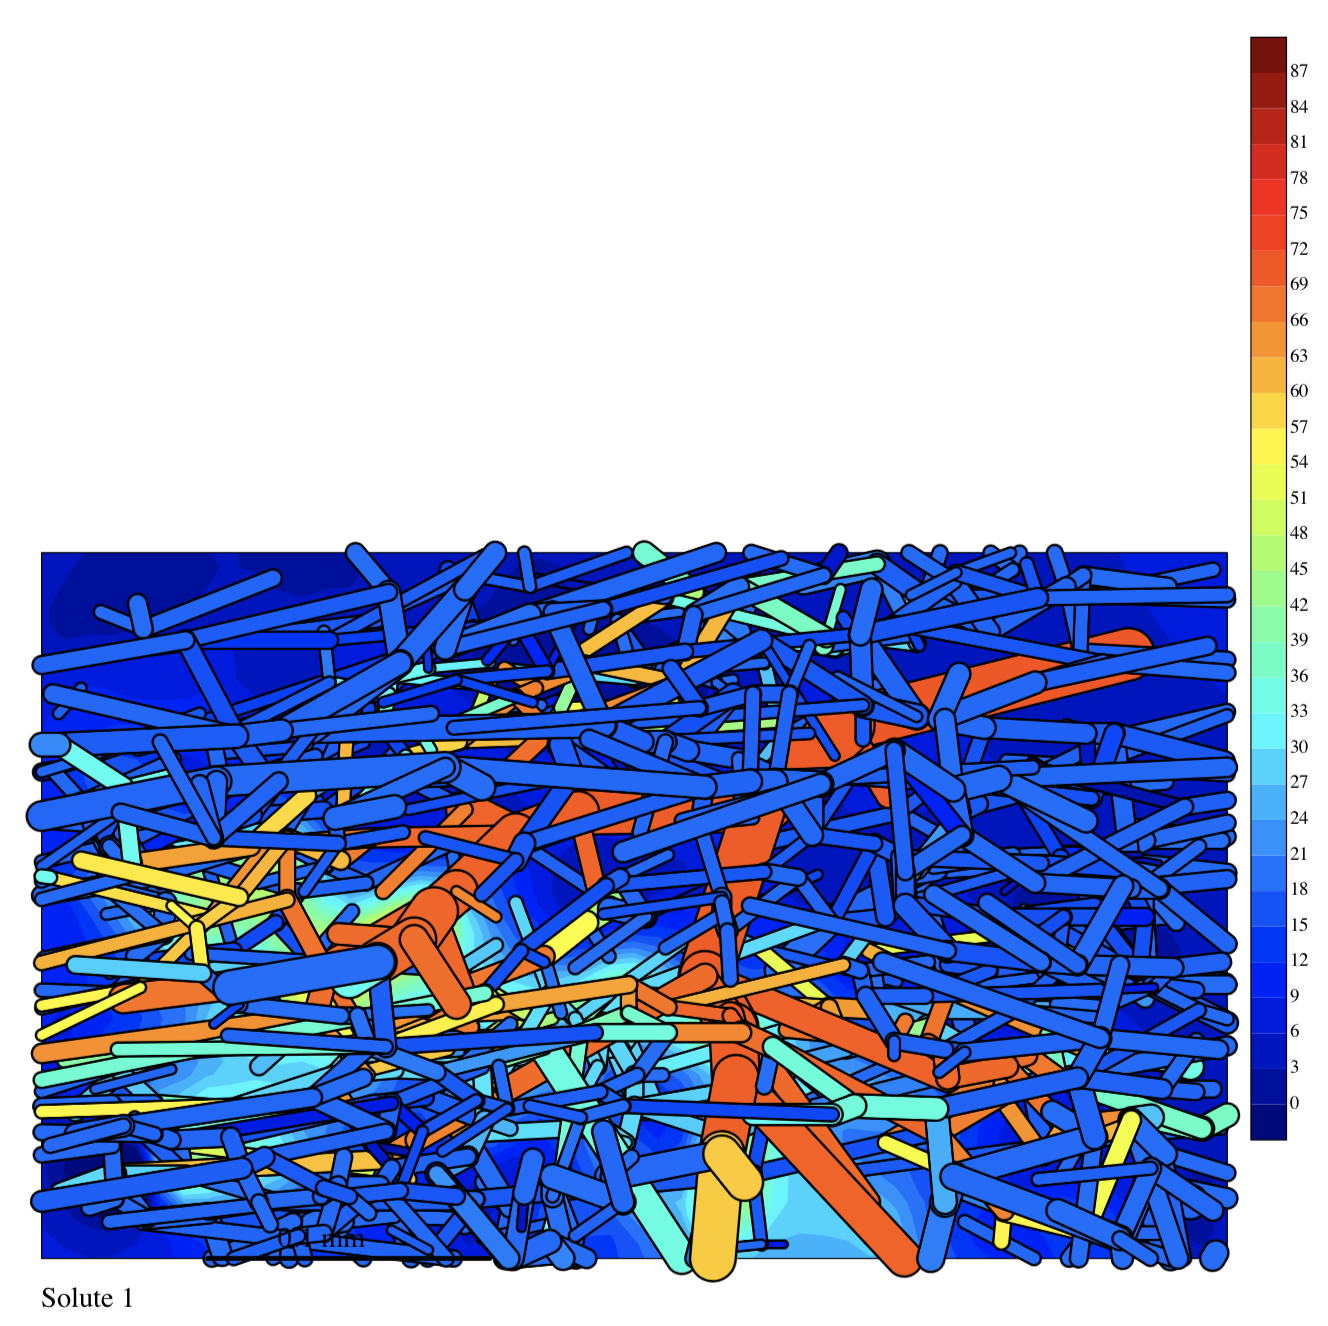
\includegraphics[width=170mm]{Contour_Cardiac}
\caption{Green's Contour Output for Cardiac Network}
\label{fig:Contour_Cardiac}
\end{figure}